\documentclass[letterpaper, twoside, titlepage, 11pt]{article}
\usepackage{fullpage}
\usepackage{graphicx}
\usepackage{hyperref}
\usepackage{subfigure}
\usepackage{url}
\usepackage{titling}

% This is here so we can have a fancier title page than LaTeX gives us by default
\newcommand{\department}[1]{%
  \gdef\dept{#1}}
\newcommand{\dept}{}
\renewcommand{\maketitlehookd}{%
\par\noindent \dept }

\title{
	smrt: A 3D Media Center User Interface
	\\
	System Architecture
}
\author{
	Cory Maccarrone  \\ {\small \href{mailto:Cory.Maccarrone@colorado.edu}{Cory.Maccarrone@colorado.edu}}
\and
	Daniel Seikaly   \\ {\small \href{mailto:Daniel.Seikaly@colorado.edu}{Daniel.Seikaly@colorado.edu}}
\and
	Evan Sheehan     \\ {\small \href{mailto:Wallace.Sheehan@gmail.com}{Wallace.Sheehan@gmail.com}}
\and
	David Trowbridge \\ {\small \href{mailto:trowbrds@gmail.com}{trowbrds@gmail.com}}
}
% \date{}
\department{
\begin{center}
	CSCI 4308-4318. Software Engineering Project 1 \& 2 \\
	Department of Computer Science \\
	University of Colorado at Boulder \\
	2005-2006 \\
	\vspace{1.5em}
	Sun Microsystems \\
	Santa Clara, CA \\
	\vspace{1em}
	Paul Byrne \\
	{\small \href{mailto:Paul.Byrne@Sun.COM}{Paul.Byrne@Sun.COM}} \\
	\vspace{1em}
	Hideya Kawahara \\
	{\small \href{mailto:Hideya.Kawahara@Sun.COM}{Hideya.Kawahara@Sun.COM}}
\end{center}
}

\begin{document}
\maketitle

\raggedbottom

\pagenumbering{roman}

\hspace{1em}
\pagebreak

\tableofcontents
\listoffigures
\pagebreak

\hspace{1em}
\pagebreak

\pagenumbering{arabic}

\documentclass[letterpaper, notitlepage, 11pt]{article}
\usepackage[body={6in, 8in}, left=1in, right=1in, top=1in, bottom=1in]{geometry}
\usepackage{fancyhdr}

\pagestyle{empty}

\begin{document}
\documentclass[letterpaper, notitlepage, 11pt]{article}
\usepackage[body={6in, 8in}, left=1in, right=1in, top=1in, bottom=1in]{geometry}
\usepackage{fancyhdr}

\pagestyle{empty}

\begin{document}
\documentclass[letterpaper, notitlepage, 11pt]{article}
\usepackage[body={6in, 8in}, left=1in, right=1in, top=1in, bottom=1in]{geometry}
\usepackage{fancyhdr}

\pagestyle{empty}

\begin{document}
\input{../lib/project-proposal}
\end{document}

\end{document}

\end{document}

\section{Introduction}
As a company, one of Sun Microsystems' objectives is to innovate the world of
computing. To this end, Sun created Project Looking Glass to explore the field
of 3D user interfaces and determine what improvements in user interaction can be
made by taking advantage of the third dimension. Through Project Looking Glass,
Sun hopes to begin redefining how people think of user interfaces and create
useful design concepts for a 3D computing environment. At the moment, Looking
Glass consists of a framework for developing 3D applications and a desktop
environment to run them alongside existing 2D applications.

The goal of this project, code named \textit{smrt}, is to create a user
interface for a home media center along the lines of TiVo, but using 3D user
interface elements within the Looking Glass environment. The name \textit{smrt}
-- pronounced ``smeert'' -- is the Czech word for ``death,'' and was primarily
chosen because it is fun to say and spell.

Figure \ref{figure:concept} presents a conceptual diagram of the overall
system.  This diagram shows how \textit{smrt} interacts with its software and
hardware environment. At the most basic level, \textit{smrt} allows a user to
browse through and play media, as well as watch or record a TV show.  To control
the system, a simple input device such as keyboard or remote control is used.
Note that this project is focused on the user interface; actual functionality
may not exist.

\begin{figure}[htb]
\centering
\includegraphics[width=4in]{figures/conceptual_overview}
\caption{Conceptual overview of the \textit{smrt} project\label{figure:concept}}
\end{figure}

There are two design issues addressed by this document: the user interface and
the implementation. Section \ref{section:ui} describes the proposed user
interface for \textit{smrt} and briefly discusses how the user interacts with
the user interface components. A high-level design of the software is given in
Section \ref{section:modules}. It defines the modules for the system and how
they interact with one another.

\section{User Interface}
\label{section:ui}
As a project, \textit{smrt}'s purpose is to explore the possibilities of a 3D
user interface. To that end \textit{smrt} uses the third dimension to increase
visibility in the system. \textit{smrt}'s user interface is designed to display
as much information for the user so that they can find and navigate to exactly
what they are looking for with as few button presses as possible.

\subsection{Components}
There are three primary menu types that \textit{smrt} uses: ring, arc, and
cityscape. A ring menu places each menu item in a circle, as shown by Figure
\ref{figure:circlemenu}. Items in the ring menu are sized according to position
to give the appearance of depth; the item closest to the user is the currently
highlighted one. Because ring menus are cyclic, the user will have at most
$\frac{n}{2}$ clicks to get to any item in the menu, where $n$ is the number of
items in the menu.

\begin{figure}[htb]
\begin{center}
\mbox{
	\subfigure[Ring Menu]{
		\label{figure:circlemenu}
		\includegraphics[width=0.25\textwidth]{figures/circle_menu_1}
	}
	\quad \quad
	\subfigure[Arc Menu]{
		\label{figure:arcmenu}
		\includegraphics[width=0.25\textwidth]{figures/arc_menu}
	}
	\quad \quad
	\subfigure[Cityscape]{
		\label{figure:cityscape}
		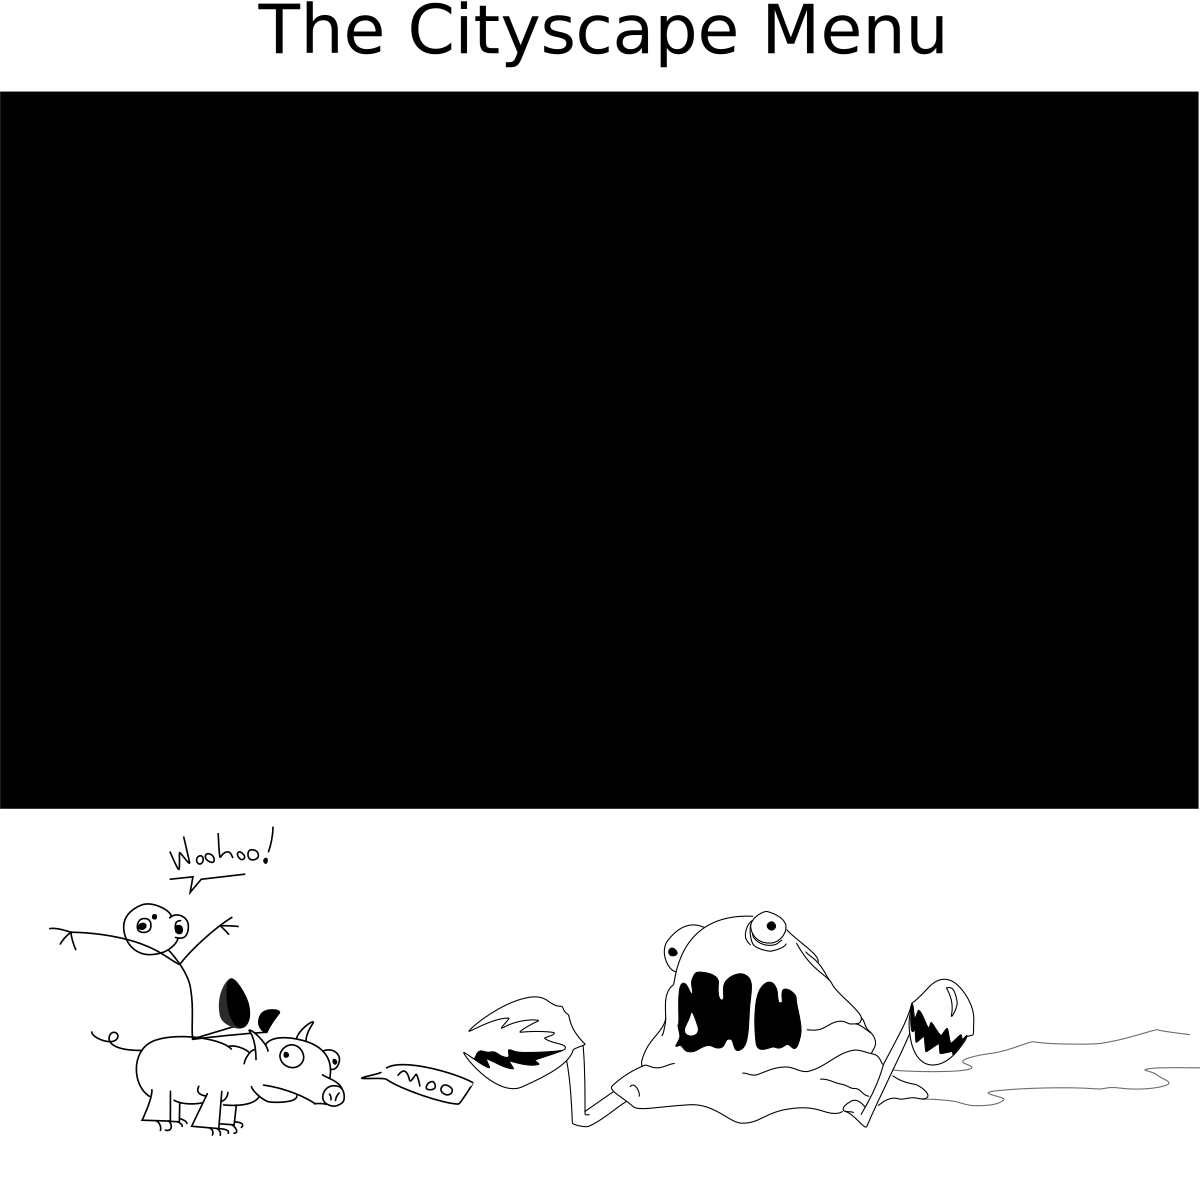
\includegraphics[width=0.25\textwidth]{figures/cityscape}
	}

}
\caption{
	Mock-ups of the three main user interface components.
}
\label{figure:mockups}
\end{center}
\end{figure}

An arc menu is similar to a normal menu that presents the menu items as a list.
Figure \ref{figure:arcmenu} shows an example of an arc menu. Like the ring menu,
the appearance of depth is created in the menu by sizing the menu items
according to position, and the closest item in the arc menu is the currently
selected one.

The cityscape menu, shown in Figure \ref{figure:cityscape} groups items into
``buildings'' -- like in \textit{Jurassic Park}. Initially, it gives the user a
coarse view of all the items in the entire menu, even when the menu is very
large.  The user can move quickly to the ``building'' containing the desired
item, making it much easier to navigate a large menu.

Both the ring menu and the cityscape menu shown in Figure \ref{figure:mockups}
present the user with all available options in a coherent manner. Thus, the user
can find the object of his or her desire without having to scroll to items off
screen.  The ring and arc menus utilize the third dimension to indicate where
the user is in the interface. The item that is closest to the user in the menu
is the selected item. As items get further from the selected item they appear
further away on the screen, making it easy for the user to determine where they
are and where they can go next.

\subsection{User Interaction}
\textit{smrt}'s main menu is a ring menu. It presents the user with a
choice of media types: TV, movies, music, etc. This menu gives the user a quick
view of the available media. Some media types will be persistent, such as a
connection to satellite TV or music stored on the computer. These items will
always appear in the menu. Other types of media, such as DVDs, will only be
displayed in the menu when they are available -- e.g., when there is a DVD in
the drive.

\textit{smrt} has two interfaces for TV; one for watching TV, and one for recording.
Both use the arc menu to select a channel.  To the left of the menu -- the gray box
in Figure \ref{figure:arcmenu} -- \textit{smrt} displays whatever is on the currently
selected channel.  Beneath this preview is program information, including the title
of the current show and a short schedule for the near future.  When recording, this
leads to an arc menu providing different recording options.

\textit{smrt} uses a cityscape menu for browsing files such as music, movies, or
recorded TV programs. The grouping of files performed by the cityscape menu
allows the user to more easily handle large media collections.

\section{High-level Modular Decomposition}
\label{section:modules}
The core of \textit{smrt} consists of several different modules that work together
to present an interface to the user and control the content on the screen.  Figure
\ref{figure:modules} shows a pictorial view of the modules.

\begin{figure}[htb]
\centering
\includegraphics[width=4in]{figures/modules}
\caption{Pictorial view of the module interaction in \textit{smrt}\label{figure:modules}}
\end{figure}

\subsection{State Controller}
The State Controller manages the global state of the system.  It receives events
from Looking Glass and dispatches them unmodified to other objects depending on
the current context.  Context is an interface which both Menus and Applications
implement.

The State Controller maintains a stack of Menus.  Menus can ask the State
Controller to push a new menu, pop the current menu or launch an application.
The Application Manager notifies the State Controller when an application
quits so that it can restore the top menu.  The top of this stack is the
current context of the State Controller, and has all input events routed to
it.

\subsection{Menus}
The Menu interface in \textit{smrt} is the basic method through which options
are presented to the user.  Menus are instantiated by and receive events from
the state controller.  When the user selects an option, the Menu tells the
state controller to change the basic state of the system.

Because some menus can also do things like display previews, they can launch
external programs through the Application Manager.  When the menu closes, it
asks the Application Manager to close the program.

\subsection{Application Manager}
The Application Manager's job is to launch external programs and position
them on the screen as desired.  This allows \textit{smrt} to take advantage of
existing media player applications.  The Application Manager also takes care
of terminating programs and restarting programs that cause problems.

\section{Summary}
\textit{smrt}'s user interface consists primarily of three menu types: ring,
arc, and cityscape. These menus are designed to increase visibility and reduce
the number of button presses required to navigate the system. As the user
navigates the system using this interface the information increases in
specificity, allowing the user find his way quickly to the information he
desires.

The system architecture for \textit{smrt} is split into three major components:
The State Controller, the Application Manager and a Menu interface.  These
components interact to provide the functionality defined in
\textit{Initial Requirements}.

% This has been a very high-level view of the initial thoughts on a system architecture
% for \textit{smrt}. It should serve as a beginning from which to start prototyping and
% to explore a more detailed design.


\end{document}
